\documentclass[fleqn,11pt,openany]{book}

% These two need to be set before including scirun style package
\title{Seg3D Basic Functionality}
\author{Jess Tate, Brett Burton}

% INCLUDE Seg3D STYLE DOCUMENT
\usepackage{seg3d}
\usepackage{marvosym}
\usepackage[rightcaption]{sidecap}
\usepackage{multirow}


\begin{document}

%% starting from SCIRun Doc wiki
%% http://software.sci.utah.edu/SCIRunDocs/index.php/CIBC:Documentation:SCIRun:Tutorial:BioPSE


% CREATE TITLE PAGE --------------------------------------------------
\maketitle

% CHAPTERS ---------------------------------------------------------------

\chapter{Overview}
\label{sec:overview}

\begin{introduction}
This document is meant as a basic reference and walkthrough of the Seg3D layout and functionality.  Specifically, every tool, filter and feature of the software will be addressed in a brief manner.

Note:  If you are looking for a refresher on the available keyboard and mouse shortcuts, there is a list under the `Help' menu of the Seg3D.  
\end{introduction}

\section{About Seg3D}

\begin{figure}
\scalebox{0.3}{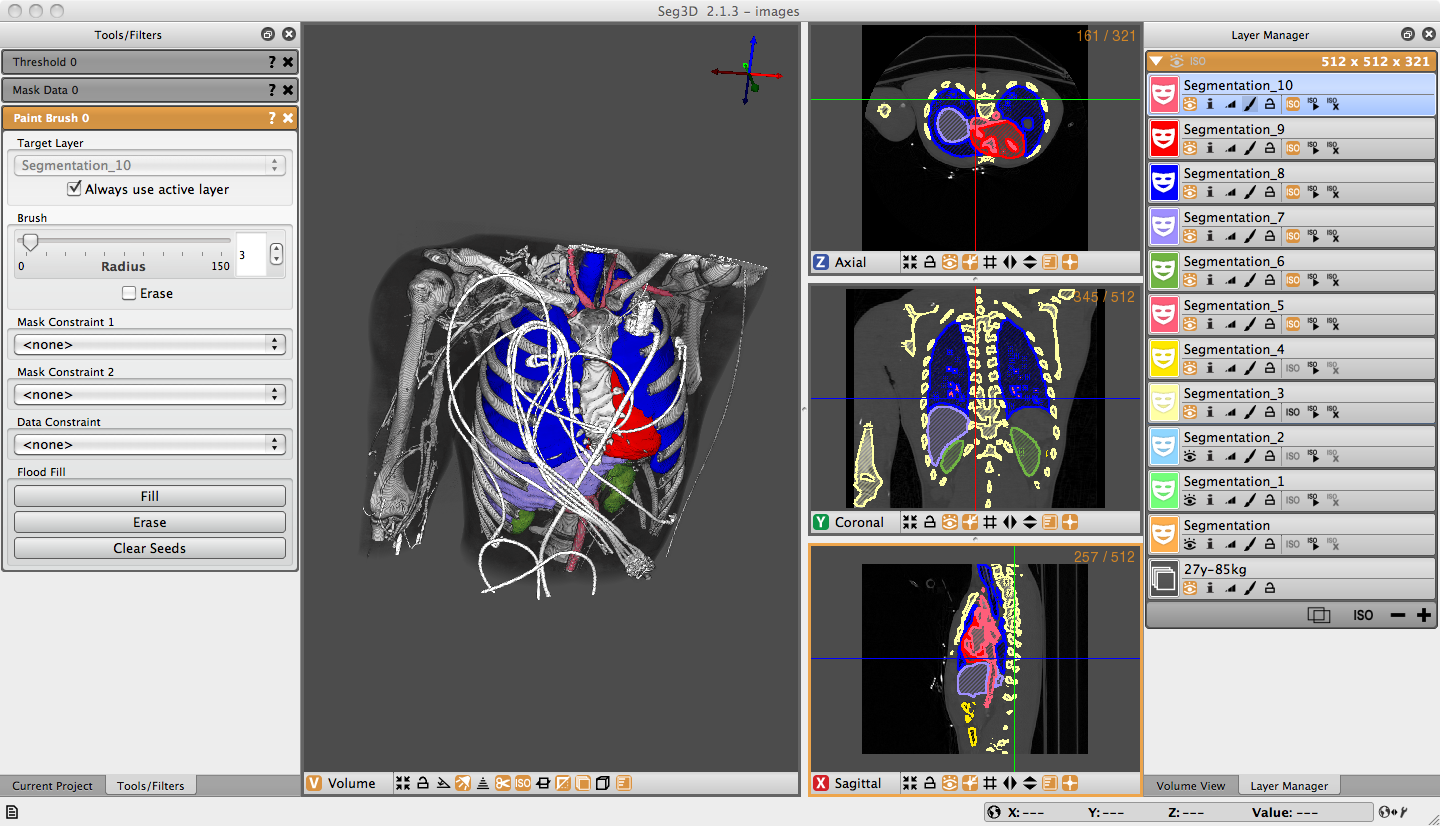
\includegraphics{Seg3DBasicFunctionality_figures/layout.png}}
\caption{Seg3D in use.}\label{fig:layout}
\end{figure}

Seg3D is a lightweight software tool developed for use in visualizing and segmenting image data.  The core intended use of Seg3D involves loading 3D scalar data, such as MRI or CT scans, and generating labels mask to identify various regions of interest in the original image data.  Seg3D facilitates the process using interactive tools such as image processing filters and manual masking techniques.  

In addition to manual segmenting, the current version of Seg3D includes some features that facilitate automated segmenting.  Provenance is a recently added feature which tracks the steps used to create label masks.  This feature allows the user to then repeat the same sets with different parameters using the python and controller windows.  Future extensions of these capabilities will allow for scripting in the terminal and porting to other programs such as SCIRun and Vistrails.

Seg3D is an crucial element of our software suite also involving BioMesh3D and SCIRun that make possible the development of image based computational models.  Label masks generated with Seg3D are used in other software  for such applications as 3D visualization or computational modeling.  BioMesh3D requires a segmentation like those from Seg3D to generate high quality, multi-material computational meshes.  SCIRun is a modular problem solving environment that generates and runs visualization and simulation tasks on segmentations from Seg3D and meshes from BioMesh3D.  This interaction makes Seg3D a key step in image based modeling.

\section{Software requirements}

\subsection{Seg3D \SegthreeDVersion}

Seg3D is distributed as a binary download for Linux, Windows, and OS X. Please visit the SCI software portal ({http://4software.sci.utah.edu} ) to download the latest Seg3D binary. 

%---------------------------------------------


\chapter{Welcome Screen}
\label{sec:welcome}

\begin{introduction}
Anytime you start Seg3D, users are first presented with the Seg3D welcome screen.  As seen in Figure~\ref{fig:welcome}, the welcome screen consists of the Seg3D splash screen and a menu displaying the available options for starting and continuing a segmentation in Seg3D.  The included options are to load a recent project, open existing project, start a new project, quickly open a file for viewing, and to quit Seg3D.  These options are the same as some of the options in the `File' menu which are explained in this chapter as well as Sec.~\ref{sec:file}.
\end{introduction}

\begin{figure}
\scalebox{0.3}{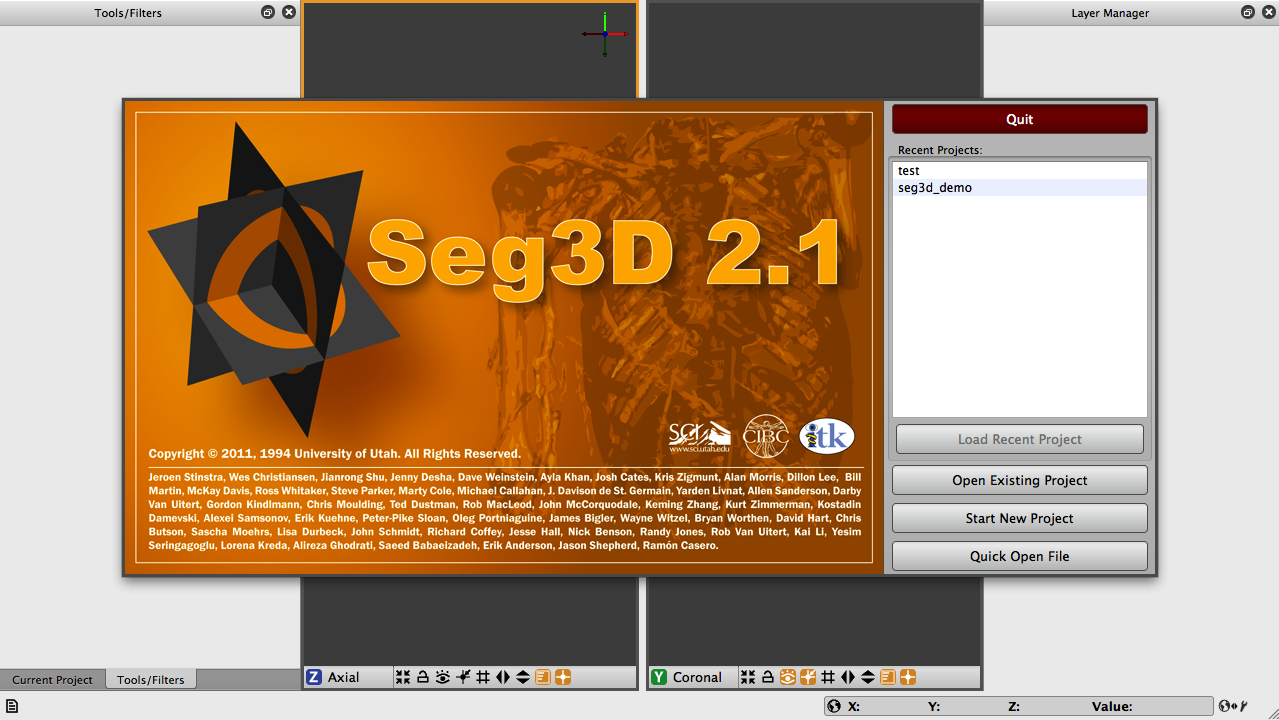
\includegraphics{Seg3DBasicFunctionality_figures/welcome_screen.png}}
\caption{Seg3D welcome screen}\label{fig:welcome}
\end{figure}


\section{Load Recent Project}

This option allows the users to quickly open a project recently opened in Seg3D.  The list of recent projects is shown in the text box above the `Load Recent Project' button (see Figure~\ref{fig:welcome}).  This option will be unavailable unless one of the recent projects in the list is selected.  Updating or reinstalling Seg3D may erase the saved list of recent projects even though the projects still exist.  

\section{Open Existing Project}

This option is the same as `File:Open Project' (sec~\ref{sec:openproject}).  It will open a dialogue window to allow the user to choose an existing *.s3d or *.seg3dproj file to load into Seg3D.  

\section{Start New Project}

This option is the same as `File:New Project' (sec~\ref{sec:newproject}).  It will display the New Project Wizard (Figure~\ref{fig:newproject}), allowing the user to choose a project name and location so that the project can be saved easily and automatically.  

\section{Quick Open File}

This option is the same as `File:Import Layer From Single File...' (sec~\ref{sec:importsinglefile}).  You may choose a file to load into Seg3D for viewing.  All of the filters and tools will be available, but the project can not be saved automatically until a project name is created by using the `File: Save Project As' (sec~\ref{sec:saveprojectas}). 
\\
\\
This option currently does not allow the opening of image stacks.

\section{Quit}

This option will quit Seg3D.  This exist for the rare occasion that you accidentally open Seg3D.  

%-------------------------------------


\chapter{Seg3D Viewer}
\label{sec:viewer}

\begin{introduction}
The Seg3D viewer is the main interface between the users and the software.  This viewer is meant to be highly interactive and intuitive.  Using a combination of mouse functions, keyboard shortcuts, and visual buttons the users can quickly visualize and segment data.  This chapter will describe the functionality of several aspects of the Seg3D viewer including the overall layout of the interface, 2D slice viewer, 3D volume viewer, and the various viewing options available.
\end{introduction}



\begin{figure}[h!]
\scalebox{0.3}{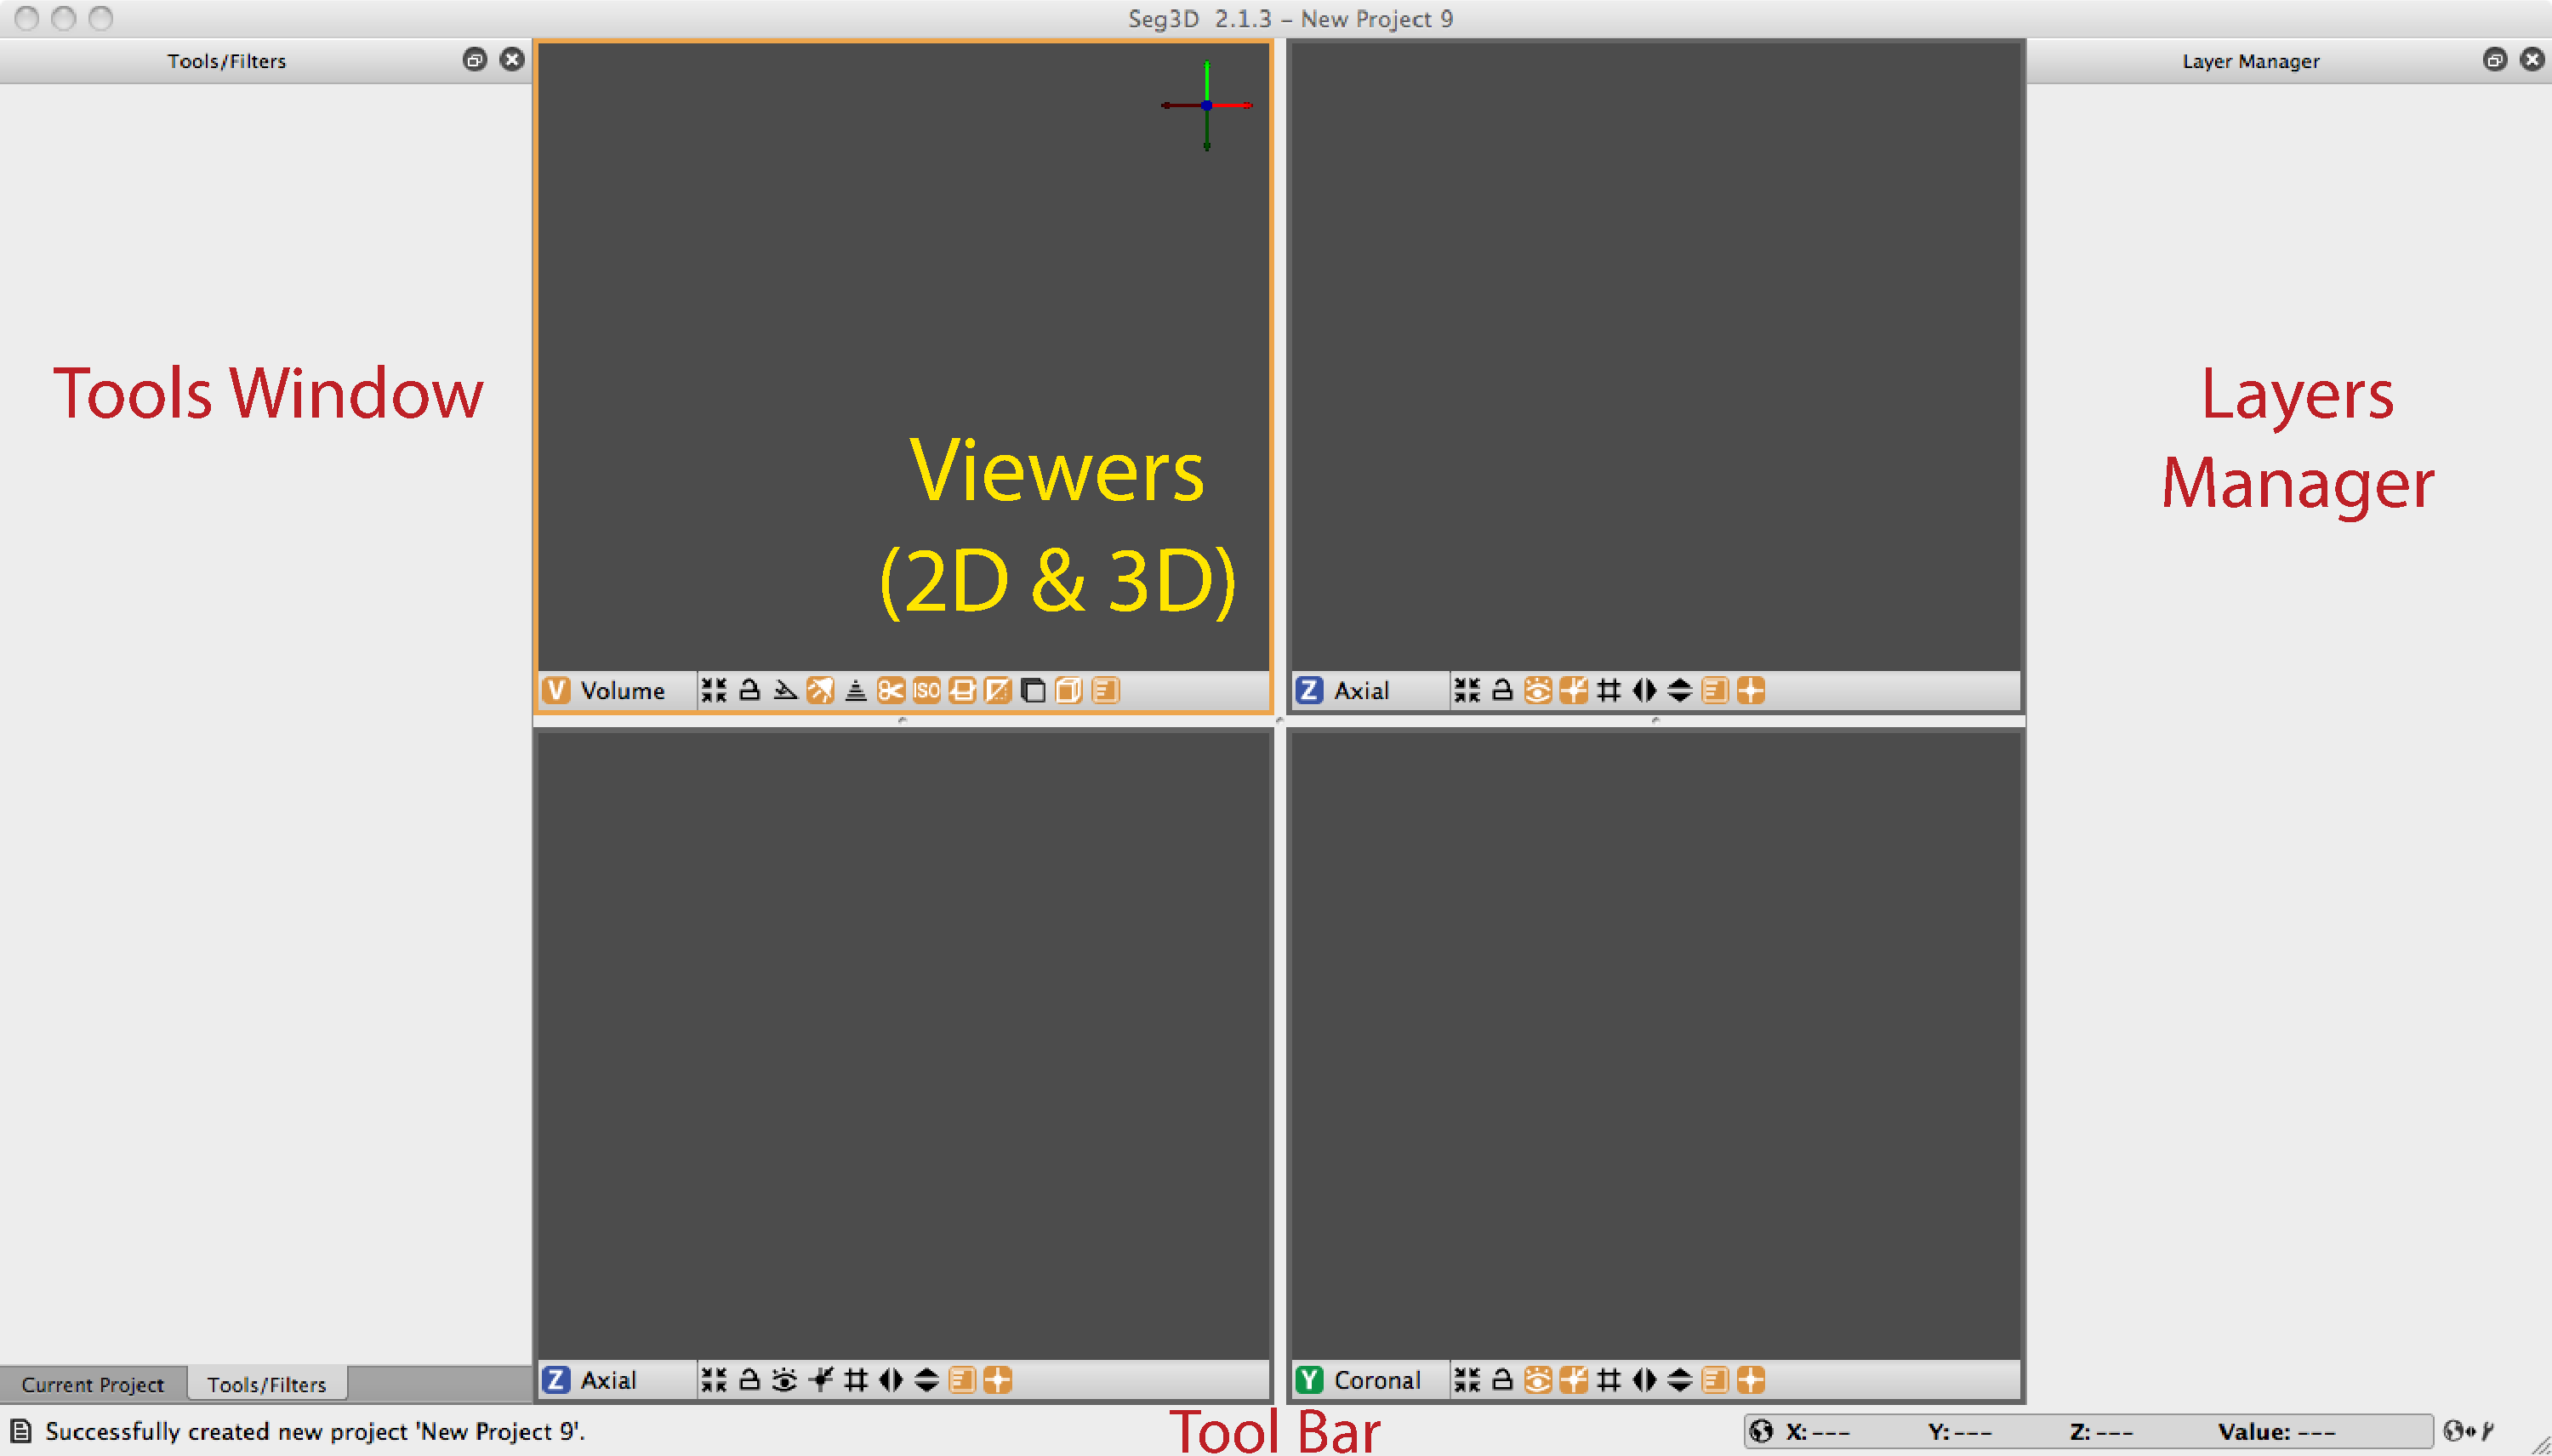
\includegraphics{Seg3DBasicFunctionality_figures/layout_blank.pdf}}
\caption{Seg3D interface}\label{fig:blank}
\end{figure}

The default layout when Seg3D is opened and a new project is created is shown in Figure~\ref{fig:blank}.  As seen from the image the interface for Seg3D consists of a number of viewers (both 2D and 3D), windows to control the functionality of Seg3D, and a tool bar at the bottom of the screen.  

\section{Controlling Windows}
\label{sec:window_control}

The windows on docked the side of the screen can be any of five windows explained in Chapter~\ref{sec:windows} (Project, Tools, Layer Manager, Volume Viewer, and Provenance windows).  Each of these widows can be closed by pressing on the close button \scalebox{0.5}{
\includegraphics{Seg3DBasicFunctionality_figures/close_window.png}} and opened by choosing the window from the `Window' menu or using hot key.  When opened, the window will appear in the last location used, or the default if never opened.  The windows can also be detached from the side (by pressing the detach button \scalebox{0.5}{
\includegraphics{Seg3DBasicFunctionality_figures/dock.png}} and reattached to the side by moving the window close to the side of the Seg3D window, or by double clicking on the window header.  Any detached window can be moved by clicking and dragging on the window header and resized by clicking and dragging on the corner of the window.  Attached windows can also be resized by clicking and dragging on border between it and the viewing panels, but are more limited in the changes allowed.  

\section{Viewer Panels}

As seen in Figure~\ref{fig:blank}, there are a number of viewer panels in Seg3D, though the exact number can be set (see Sec.~\ref{sec:viewing}).  Each of these viewer windows can be changed in size and in type.  The type options are: volume, axial, sagittal, and coronal. The names of the 2D planes can be changed by the user in preferences (Sec.~\ref{sec:preferences}).  You can change the view of each pane by clicking on the view name and choosing the view to change it too.  This is a drop down menu, so you can scroll over the name and the view will also change.  There are also shortcuts to change views (V--Volume, X--Sagittal, Y--Coronal, and Z--Axial) There are several icons in each view panel, as well as mouse and keyboard shortcuts.  The controls for each of the 2D viewers will be described below, as will the controls for the 3D volume viewer.

\subsection{2D Slice Viewer}

Tables~\ref{tab:2dmouse}~\&~\ref{tab:2dkey}  show the mouse and keyboard actions which can be used to control the visualization and manipulation of image and segmentation data.  Though these functions are general, there are tools which used these functions for specify purposes or may otherwise block a couple of these functions, the most prominent example is the scroll wheel in the paint brush tool is used to change brush size.  In this case, you can still scroll through slices by holding shift.  In all cases, an alternative is given in the software.  Also presented in this section is a list and description of the icons presented in the 2D slice viewer (Table~\ref{tab:2dicons}).

\begin{table}[h!]
\label{tab:2dmouse}
\caption{List of mouse functions in the 2D viewers}
\begin{tabular}{|l|l|}
\hline
{\bf Mouse Command} & {\bf Function}\\
\hline
left button drag & Modify brightness and contrast.  \\ &Vertical is contrast, horizontal is brightness. \\
\hline 
scroll up/down & Move up/down a slice\\ &Note: using shift maybe needed while using some tools (like paint brush)\\
\hline
cmd/crtl+right button & Move slices in other planes to intersect at cursor.\\  &Viewers must have the picking icon enabled (Figure~\ref{fig:pick}).\\
\hline
shift+left button drag & Zan view\\
shift+right button drag & Zoom view in/out\\
\hline
\end{tabular}
\end{table}

\begin{table}[h!]
\label{tab:2dkey}
\caption{List of keyboard actions in the 2D viewers}
\begin{tabular}{|l|l|}
\hline
{\bf Keyboard Action} & {\bf Function}\\
\hline
up arrow,$>$ & move up one slice\\
down arrow,$<$ & move down one slice\\
\hline
shift+up arrow,shift+$>$ & Jump up n slices (set n in preferences)\\
shift+down arrow,shift+$<$ & Jump down n slices (set n in preferences)\\
\hline
left/right arrow & Change active layer to previous/next layer\\
\hline
SPACE & Toggle layer visibility on/off (active layer)\\
\hline
G & Toggle grid visibility\\
\hline
P & Toggle picking state\\
\hline
T & Toggle overlay visibility\\
\hline
L & Toggle lock viewer (to other locked views of the same type)\\
\hline
\end{tabular}
\end{table}

\begin{table}[h!]
\label{tab:2dicons}
\caption{List of icons and actions in the 2D viewers}
\begin{tabular}{|l|l|}
\hline
{\bf Icon} & {\bf Function}\\
\hline
\multirow{2}{*}{ 
\includegraphics[width=0.05\textwidth]{Seg3DBasicFunctionality_figures/AutoViewOff.png} }
& Autoview Icon: This icon forces the panel to fit the objects in viewer with \\
& maximum size.\\
\hline
\multirow{3}{*}{ 
\includegraphics[width=0.05\textwidth]{Seg3DBasicFunctionality_figures/LockOff.png} }
& Lock View Icon: This icon toggles the viewer lock on the panel (shortcut: L). \\ 
& Any changes to any locked viewers will change all the views.  Viewers must \\
& be the same type and each must be locked to use this funtion.\\
\hline
\multirow{2}{*}{ 
\includegraphics[width=0.05\textwidth]{Seg3DBasicFunctionality_figures/VisibleOff.png} }
& Visibility Icon: This icon toggles the visibility of the plane in the 3D volume \\
& viewer.\\
\hline
\multirow{3}{*}{ 
\includegraphics[width=0.05\textwidth]{Seg3DBasicFunctionality_figures/PickingOff.png} }
& Picking Icon: This icon toggles the ability of other planes to pick the slice to \\
& view in the panel.  Only one viewer can have this option enabled.  if only on \\
& of a type of plane, this cannot be disabled.\\
\hline
\multirow{2}{*}{ 
\includegraphics[width=0.05\textwidth]{Seg3DBasicFunctionality_figures/GridOff.png} }
& Grid Icon: This icon toggles the visibility of the grid in the viewer.\\
& \\
\hline
\multirow{2}{*}{ 
\includegraphics[width=0.05\textwidth]{Seg3DBasicFunctionality_figures/FlipHorizOff.png} }
& Flip Horizontal Icon: This icon will horizontally flip the visualization \\
& of the slices in the viewer.\\
\hline
\multirow{2}{*}{ 
\includegraphics[width=0.05\textwidth]{Seg3DBasicFunctionality_figures/FlipVertOff.png} }
& Flip Vertical Icon: This icon will vertically flip the visualization of \\
& the slices in the viewer.\\
\hline
\multirow{2}{*}{ 
\includegraphics[width=0.05\textwidth]{Seg3DBasicFunctionality_figures/OverlayOff.png} }
&  Overlay Icon: This icon will toggle the visibility of the overlay on \\
& the viewer.  This will allow unobstructed viewing of the slices.\\
\hline
\multirow{2}{*}{ 
\includegraphics[width=0.05\textwidth]{Seg3DBasicFunctionality_figures/PickingLinesOff.png} }
& Picking Lines Icon: This icon toggles the visibility of the picking\\
& lines (shows other slices) in the viewing panel.\\
\hline
\end{tabular}
\end{table}

\subsection{3D Volume Viewer}

Though there is no segmentation that can be performed in the 3D volume viewer, it is a very useful function in Seg3D.  It allows the user to see the 3D representation of the original and segmented data.  There are many objects that can be viewed in the 3D viewer such as the 2D slices in 3D, isosurfaces of the segmented data, volume rendering of the image data,  depth cues, and clipping planes.  The purpose of this viewer is to allow you to view your data in as many ways as possible to facilitate segmentation.

\begin{table}[h!]
\label{tab:3dmouse}
\caption{List of mouse functions in the 3D volume viewer}
\begin{tabular}{|l|l|}
\hline
{\bf Mouse Command} & {\bf Function}\\
\hline
left button drag & Pan scene\\
\hline
middle button drag & Rotate scene\\
\hline
right button drag & Zoom in/out on scene\\
\hline
\end{tabular}
\end{table}

\begin{table}[h!]
\label{tab:2dkey}
\caption{List of keyboard actions in the 3D volume viewer}
\begin{tabular}{|l|l|}
\hline
{\bf Keyboard Action} & {\bf Function}\\
\hline
H & Toggle volume lighing\\
\hline
I & Toggle isosurface visibility\\
\hline
T & Toggle overlay visibility\\
\hline
L & Toggle lock viewer (to other locked views of the same type)\\
\hline
\end{tabular}
\end{table}

\begin{table}[h!]
\label{tab:3dicons}
\caption{List of icons and actions in the 3D viewer}
\begin{tabular}{|l|l|}
\hline
{\bf Icon} & {\bf Function}\\
\hline
\multirow{2}{*}{ 
\includegraphics[width=0.05\textwidth]{Seg3DBasicFunctionality_figures/AutoViewOff.png} }
& Autoview Icon: This icon forces the panel to fit the objects in viewer with \\
& maximum size.\\
\hline
\multirow{3}{*}{ 
\includegraphics[width=0.05\textwidth]{Seg3DBasicFunctionality_figures/LockOff.png} }
& Lock View Icon: This icon toggles the viewer lock on the panel (shortcut: L). \\ 
& Any changes to any locked viewers will change all the views.  Viewers must \\
& be the same type and each must be locked to use this funtion.\\
\hline
\multirow{2}{*}{ 
\includegraphics[width=0.05\textwidth]{Seg3DBasicFunctionality_figures/AlignOff.png} }
& Snap to Axis Icon: This icon will move the scene so that the viewing angle is \\
& aligned with the nearest axis.  This will effectively ``straighten'' the scene.\\
\hline
\multirow{3}{*}{ 
\includegraphics[width=0.05\textwidth]{Seg3DBasicFunctionality_figures/LightOff.png} }
& Lighting Icon: This icon toggles the lighting in the 3D viewer.  With the \\
& lighting disable, the images will be shaded as if they were flat, i.e., no \\
& shading.\\
\hline
\multirow{3}{*}{ 
\includegraphics[width=0.05\textwidth]{Seg3DBasicFunctionality_figures/FogOff.png} }
& Depth Cue Icon: This icon toggles the depth cue for the 3d viewer.  This depth\\
& cue acts as fog, blending objects further from the camera into the background.\\
& Fog parameters can be changed in the volume view window (Sec.~\ref{sec:fog}).\\
\hline
\multirow{3}{*}{ 
\includegraphics[width=0.05\textwidth]{Seg3DBasicFunctionality_figures/ClipOff.png} }
& Clipping Icon: This icon toggles the viewing of the clipping planes in the 3D\\
& viewer.  Clipping planes must be created before they can be seen in the volume\\
& viewer (Sec.~\ref{sec:clipping}).\\
\hline
\multirow{3}{*}{ 
\includegraphics[width=0.05\textwidth]{Seg3DBasicFunctionality_figures/IsosurfaceVisibleOff.png} }
& Isosurface Visibility Icon: This icon toggles visibility of the isosurfaces in the\\
& 3D viewer.  This functions effects all the isosurfaces are declared visible in\\
& the layer manager.\\
\hline
\multirow{2}{*}{ 
\includegraphics[width=0.05\textwidth]{Seg3DBasicFunctionality_figures/SlicesVisibleOff.png} }
& Slice Visibility Icon: This icon toggles visibility of the slices in the 3D \\
& viewer.\\
\hline
\multirow{3}{*}{ 
\includegraphics[width=0.05\textwidth]{Seg3DBasicFunctionality_figures/InvisibleSlicesVisibleOff.png} }
& Invisible Slice Visibility Icon: This icon toggles visibility of the invisible\\
& slices in the 3D viewer.  Invisible slices are left when 2D viewers are \\
& destroyed.\\
\hline
\multirow{3}{*}{ 
\includegraphics[width=0.05\textwidth]{Seg3DBasicFunctionality_figures/VolumeRenderingOff.png} }
& Volume Rendering Visibility Icon: This icon toggles visibility of the Volume\\
& Rendering in the 3D viewer.  Volume Rendering must first be created in the\\
& Volume View window (Sec.~\ref{sec:volumerendering})\\
\hline
\multirow{2}{*}{ 
\includegraphics[width=0.05\textwidth]{Seg3DBasicFunctionality_figures/VolumeVisibleOff.png} }
& Volume visibility Icon: This icon toggles visibility of the borders of the active\\ 
& layer in the 3D viewer.\\
\hline
\multirow{2}{*}{ 
\includegraphics[width=0.05\textwidth]{Seg3DBasicFunctionality_figures/OverlayOff.png} }
&  Overlay Icon: This icon will toggle the visibility of the overlay on \\
& the viewer.  This will allow unobstructed viewing of the scene.\\
\hline
\end{tabular}
\end{table}



\section{Tool Bar}

The tool bar located at the bottom of the Seg3D window contains some useful functions.  The first is the message history icon on the left side of the tool bar (Figure~\ref{fig:messagehistory}).  For more information on this window, see Sec.~\ref{sec:messagehistory}.  The other use function is on the right side of the tool bar, the information tool bar.  This tool bar can switch between displaying information about the active layer at the mouse location and a quick menu for the active layers by clicking on the switch tool button (Figure~\ref{fig:switchtool}).  

\begin{SCfigure}[20][h]
  
\includegraphics[width=0.05\textwidth]{Seg3DBasicFunctionality_figures/TextOff.png}
  \caption{Message History Icon: Opens Message History window.}
  \label{fig:messagehistory}
\end{SCfigure}

\begin{SCfigure}[20][h]
\vspace{5 pt}
  
\includegraphics[width=.08\textwidth]{Seg3DBasicFunctionality_figures/SwitchTool.png}
  \caption{Switch Tool Icon:  Switches between displaying location of mouse in the volume and the quick menu to switch between the active tools and layers.}
  \label{fig:switchtool}
\end{SCfigure}

\begin{SCfigure}[20][h]
\vspace{3 pt}
  
\includegraphics[width=.05\textwidth]{Seg3DBasicFunctionality_figures/WorldOff.png}
  \caption{World Icon:  Switches between coordinate system displayed in the information tool bar.  The options are relative (indexed) and absolute (world).}
  \label{fig:world}
\end{SCfigure}

The information toolbar will show information about the volume at the location indicated by the mouse.  As shown in Figure~\ref{fig:geometricinfo}, the information given is the x, y, and z coordinates and the value of the layer at the mouse position in the selected volume.  By clicking on the world icon (Figure~\ref{fig:world}), you may toggle between indexed values (relative) and the world values (absolute, considers spacing).  The data shown is changed when the mouse is moved, the active slice is changed, or the active layer is changed.

\begin{figure}[h!]
\scalebox{.7}{
\includegraphics{Seg3DBasicFunctionality_figures/geometric_info.png}}
\caption{Geometric Information shown in the information tool bar.}\label{fig:geometricinfo}
\end{figure}

By clicking on the switch tool icon (Figure~\ref{fig:switchtool}), the tool bar will display a quick menu for the available tools and layers instead of geometric information.  As seen in Figure~\ref{fig:quickmenu}, this menu will display the active tool and layer.  if the either is clicked, a dropped down menu will appear allowing the user to switch to an open tool or layer.  This can be especially useful in full screen mode.  

\begin{figure}[h!]
\scalebox{.7}{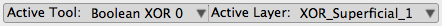
\includegraphics{Seg3DBasicFunctionality_figures/quick_menu.png}}
\caption{Quick menu shown in the information tool bar.}\label{fig:quickmenu}
\end{figure}


\section{Viewing Options}
\label{sec:viewing}

There are several options to change the layout and data viewing in Seg3D.  As mentioned before, several windows can be moved and undocked to customize the layout.  The viewing panels can also be altered so that there are virtually any number (up to sixe) and any size.  Viewing panel sizes can be adjusted by clicking and dragging on the borders.  This may change the sizes of several panels at once, but there are several different configurations available in the `View' menu at the top of the screen.  The various options are explained in the sections following.  

\subsection{Full Screen}

This is a unique and useful viewing option will cause Seg3D to use all of the real estate of whatever screen you are using.  Full screen mode will cover everything else that may be open on your desktop, including the common menus on the top and bottom of the screen.  The top tool bar will reappear if the mouse is held at the top of the screen momentarily, allowing the user to choose any tools or filters desired.  Full screen mode is enable and disabled by clicking on the option in the menu, or by using the shortcut: ctrl/cmd+F.  

\subsection{Only One Viewer}

This and the following viewing options should be self evident.  This option will show only one viewer.  This is useful if you only care about one view at a time because it maximizes screen real estate.  This one viewer can still be switch between the 3 slice orientations and the volume viewer.  

\subsection{One and One}

This will display two viewers side by side.  

\subsection{One and Two}

This will create three viewers,  one bigger one on the left and two smaller ones stacked on the right.  

\subsection{One and Three}

This is the default configuration,  though it can be changed int he preferences.  This generates four viewers, one large one on the left and three smaller ones stacked on the right.  This is a useful configuration because most people do more work in a single view, giving the user one large space to work, but use the other views as references only, so they do not take as much space.

\subsection{Two and Two}

This will generate four viewers of equal size, two on the left and right.  This is useful when you segment in multiple planes simultaneously.

\subsection{Two and Three}

This generates five viewers, two on the left and three on the right.  For when four just doesn't cut it.  

\subsection{Three and Three}

This generates six viewers, the maximum number, three on the left and right.  This is generally used when multiple planes in the same direction are needed.  These planes can be locked together as the user scrolls through them.  

\subsection{Table of Shortcuts}

\begin{table}[h!]
\label{tab:viewerkey}
\caption{Shortcuts for the various viewing options}
\begin{tabular}{|l|l|}
\hline
{\bf Keyboard Action} & {\bf Function}\\
\hline
ctrl/cmd+F & Toggle Full Screen Mode\\
\hline
alt+0 & One viewer only\\
\hline
alt+1 & One and One\\
\hline
alt+2 & One and Two\\
\hline
alt+3 & One and Three\\
\hline
alt+4 & Two and Two\\
\hline
alt+5 & Two and Three\\
\hline
alt+6 & Three and Three\\
\hline
\end{tabular}
\end{table}



%%%%%%%%%%%%%%%%%%%%%%%%%%%%%%%%%%%%%%%%%%%%%%
%---------------------------------------------------------------------------------%%%%%%%%%%%%%%%%%%%%%%%%%%%%%

\chapter{Seg3D Windows}
\label{sec:windows}

\begin{introduction}
In addition to the viewer windows discussed in the above chapter, there are several other
 windows involved in streamlining the user interface of the Seg3D software.  
 Each of these windows can be accessed through the 'Window' drop-down menu.
 By default these windows appear in certain positions defined below, but each can be undocked
 from the Seg3D interface and either left as stand alone windows or repositioned elsewhere on
 the Seg3D application (see Sec.~\ref{sec:window_control}).  
\end{introduction}

\section{Project Window}

\begin{figure}
\scalebox{0.3}{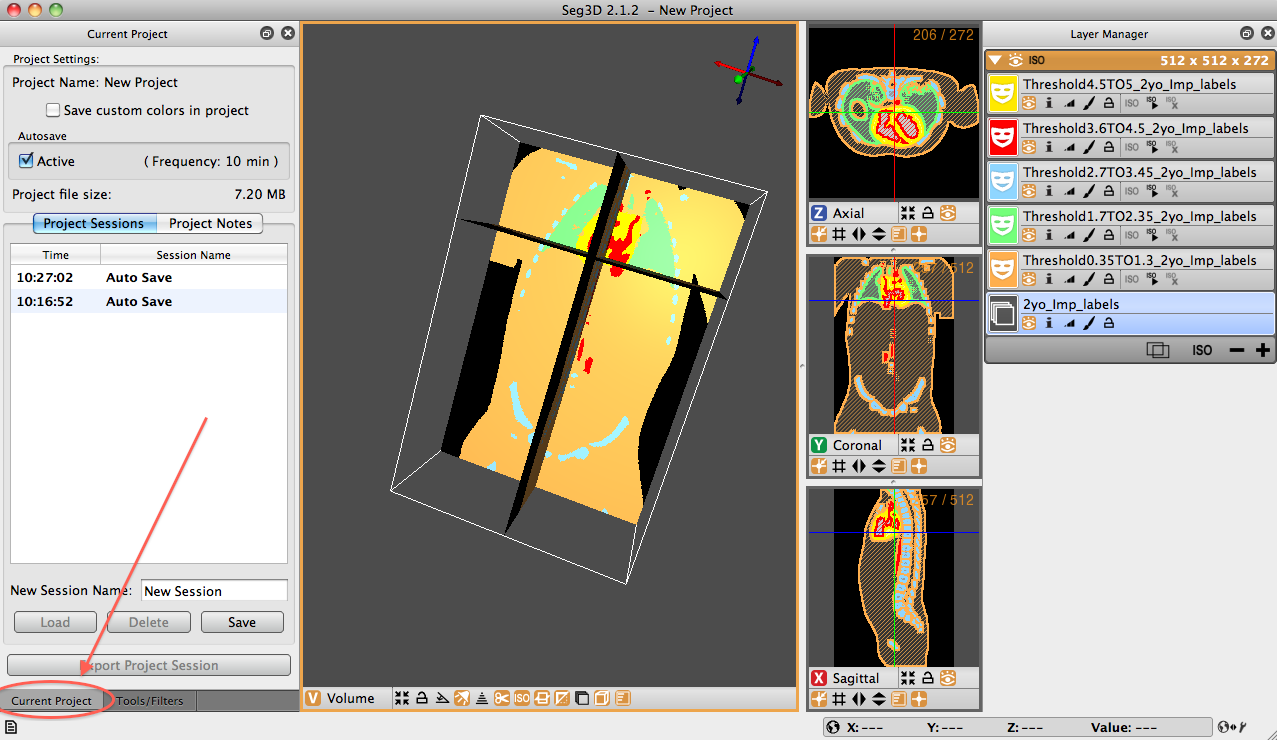
\includegraphics{Seg3DBasicFunctionality_figures/ProjectWindow.png}}
\caption{Project Window}\label{fig:ProjectWindow}
\end{figure}
The project window is one of three windows that is opened by default when Seg3D launches.  
It is located on the left side of the panel and is secondary to the default 'Tools Window' which is also 
located on the left but appears over top of the project window.  
In order to access the window, simply click the tab at the bottom of the left side named 'Current Project' (See Figure \ref{fig:ProjectWindow}) or go to the 'Window' drop down menu, de-select 
'Project Window' and reselect it.

Now you come to the 'Current Project' window.  
The window is divided into two panes.  
At the top of the window is the Project Settings pane.  
The name of the current project is listed.  
Below this is the option to 'Save custom colors in project.'  
This option allows the user to keep the defined colors assigned to specific label masks within the project.  
Below this is an 'Autosave' option. Seg3D autosaves sessions every 10 minutes by default.  
The default time between autosaves can be changed in the general Seg3D preferences.

The second pane holds the 'Project Sessions' and 'Project Notes' panels.  
The project session contains information on the saving of various sessions throughout the work-time in Seg3D - including autosaves.  
These session saves can be selected and loaded at any time.  
Loading a session save does not delete saves that came later.  
To delete, the user must explicitly select the session and push the delete button at the bottom of the pane.  
Additional sessions may also be saved with user specified names.  
The second panel of this pane (the 'Project Notes' panel) allows the user to write notes to along the way.

At any time the user can export the session to a new location - with or without a different name than the original session by clicking the 'Export the Project Session button on the bottom of the  'Current Project' window.

\section{Tools Window}
\begin{figure}[b]
\scalebox{0.3}{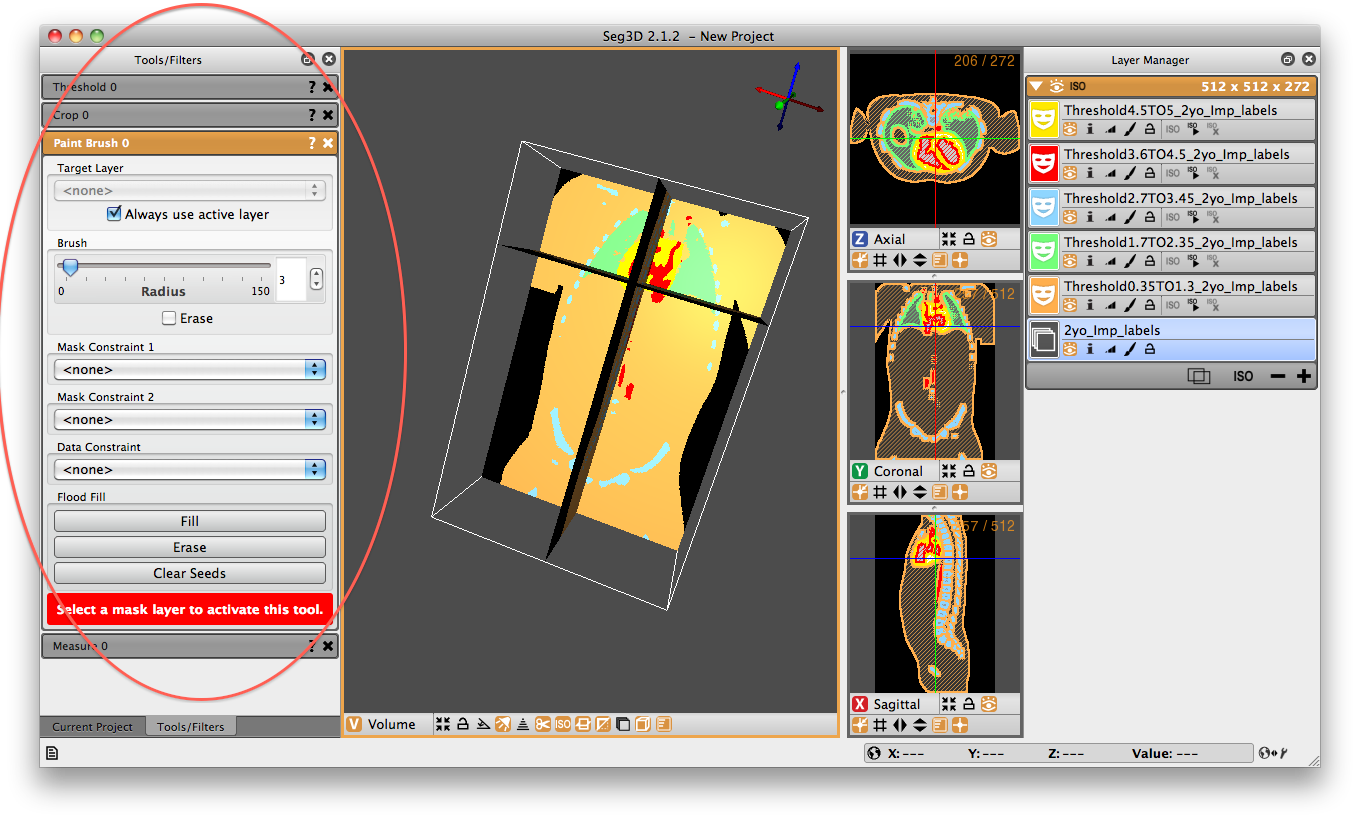
\includegraphics{Seg3DBasicFunctionality_figures/ToolWindow.png}}
\caption{Tools Window}\label{fig:ToolWindow}
\end{figure}
The tools window is another of the three windows that is opened upon Seg3D launch.  
This window is also on the left of the Seg3D panel and is, unlike the project window, is displayed when Seg3D is opened.  
Users can toggle between project and tool windows by selecting the specific tabs at the bottom of the left most window pane.

The tool window houses the current tools that the user has selected from the 'Tools' drop down menu.  
The active tool will be highlighted in orange and will be displayed.  
Inactive tools, that have been opened during the session, will be grayed out and minimized.  
To access one of the other tools, click one of the grayed out items or select it from the 'Tools' drop down menu.  
In Figure \ref{fig:ToolWindow} the 'Paint Brush' tool is active, while the 'Threshold,' 'Crop,' and 'Measure' tools are inactive.



\section{Layer Manager Window}

\begin{figure}[ht!]
\scalebox{0.3}{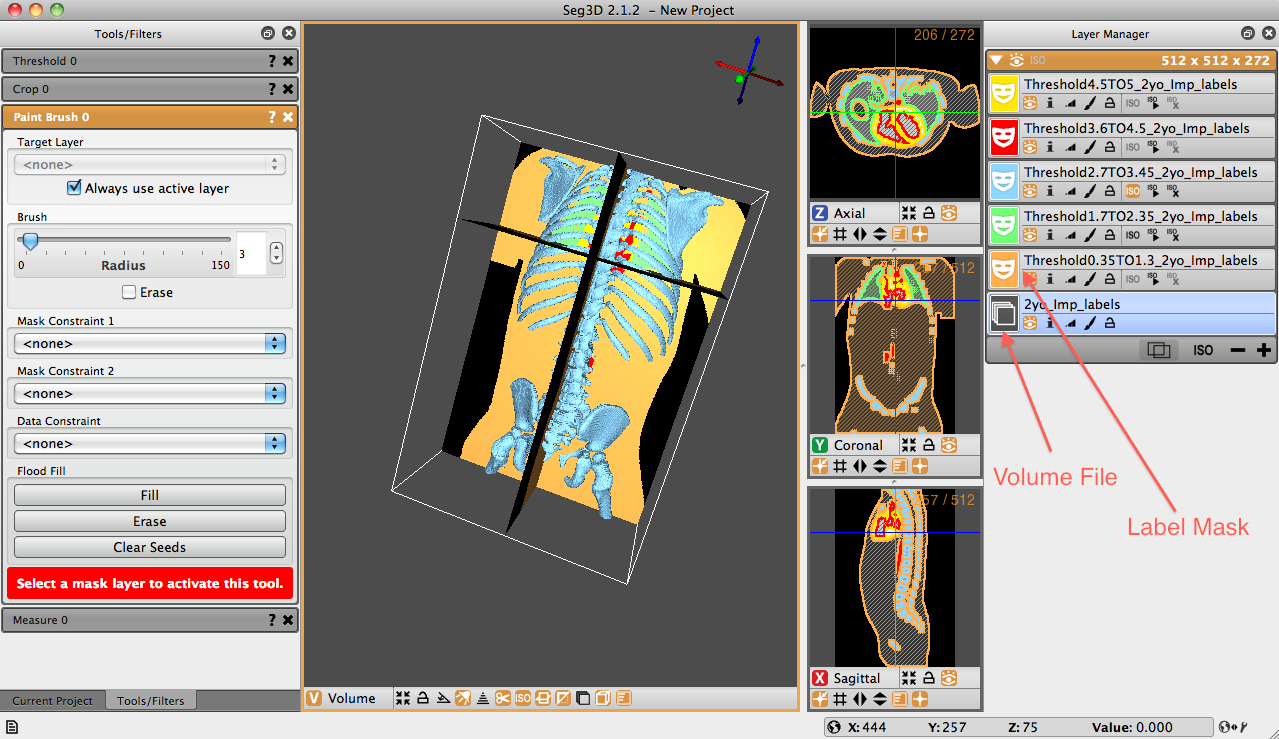
\includegraphics{Seg3DBasicFunctionality_figures/LayerWindow.png}}
\caption{Layer Manager Window}\label{fig:LayerWindow}
\end{figure}

The layer manager window is the last of the three windows that open by default upon launching Seg3D.  
This window is positioned to the right side of the Seg3D window pane and contains all of the mask and volume files involved with the session.  
If a file is not selected when Seg3D launches, this window will be blank, otherwise it will contain the volume and mask surface files associated with the opened file.

A volume file is represented by a gray image with multiple stacked planes.  
A label mask is represented by a colored icon with a white mask in the middle.  
The colors correspond to the label masks seen in the viewer windows.
Names of label masks are, by default, a conglomeration of the tools applied to the original volume.
For example, in the image Figure \ref{fig:LayerWindow} five label masks have been created from the volume file '\verb|2yo_Imp_labels|.' 
The uppermost mask (in yellow) has the name '\verb|Threshold4.5TO5_2yo_Imp_labels|.' 
This name was generated because the threshold tool, with values between 4.5 and 5, was applied to the original volume file. 
If another tool were to be applied on the yellow mask, the new mask would state the name of the tool, followed by the complete name of the yellow label mask.  
Names of masks can be manually changed by clicking the current name and typing in the desired text.

\begin{table}[h!]
\label{tab:layericons}
\caption{List of icons and actions available for each layer.}
\begin{tabular}{|l|l|}
\hline
{\bf Icon} & {\bf Function}\\
\hline
\multirow{3}{*}{ 
\includegraphics[width=0.05\textwidth]{Seg3DBasicFunctionality_figures/VisibleOff.png} }
& Visible Icon: The eye icon displays the current mask.  When the eye is \\
& highlighted the mask is visible in the view plane, when it is not, the mask \\
& is 'turned off.'\\
\hline
\multirow{2}{*}{ \includegraphics[width=0.05\textwidth]{Seg3DBasicFunctionality_figures/infoOff.png} }
& Info Icon: The 'i' icon displays information about the layer.\\
& \\
\hline
\multirow{2}{*}{ 
\includegraphics[width=0.05\textwidth]{Seg3DBasicFunctionality_figures/OpacityOff.png} }
& Opacity Icon: The histogram-looking icon allows the user to change opacity\\
& levels of the layer.\\
\hline
\multirow{2}{*}{ 
\includegraphics[width=0.04\textwidth]{Seg3DBasicFunctionality_figures/AppearanceOff.png} }
& Appearance Icon: The paintbrush-like icon allows the user to change the \\
& layer's appearance.\\
\hline
\multirow{2}{*}{ 
\includegraphics[width=0.05\textwidth]{Seg3DBasicFunctionality_figures/LockOff.png} }
& Lock Icon: The lock icon allows users to lock the layer to further editing.\\
& \\
\hline
\multirow{2}{*}{ 
\includegraphics[width=0.05\textwidth]{Seg3DBasicFunctionality_figures/IsosurfaceVisibleOff.png} }
& Isosurface Visible Icon: This icon toggles visibility of the layers isosurface.  \\
& Isosurfaces must be computed first.\\
\hline
\multirow{3}{*}{ 
\includegraphics[width=0.05\textwidth]{Seg3DBasicFunctionality_figures/IsosurfaceComputeOff.png} }
& Isosurface Compute Icon: This icon generates the isosurface for the mask.\\
& It must be clicked before the IsosurfaceMenu or IsosurfaceDelete icons\\
& become active.\\
\hline
\multirow{2}{*}{ 
\includegraphics[width=0.05\textwidth]{Seg3DBasicFunctionality_figures/IsosurfaceDeleteOff.png} }
& IsosurfaceDelete Icon: This icon deletes active isosurfaces (if the mask\\
& has one).\\
\hline
\end{tabular}
\end{table}

Each volume or mask label has  standard, associated icons below their names.  Table~\ref{tab:layericons} displays and describes each of these icons.  These icons represent tools that are available for each individual layer. 

 \begin{table}[h!]
\label{tab:layertopicons}
\caption{List of icons and actions available at the top of each layer group.}
\begin{tabular}{|l|l|}
\hline
{\bf Icon} & {\bf Function}\\
\hline
\multirow{4}{*}{ 
\includegraphics[width=0.05\textwidth]{Seg3DBasicFunctionality_figures/DownArrow.png} }
& Expanded Layer Group Icon:  This icon indicates that the layer group is \\
& visible, showing all the layers in it.  The layer group can be collapsed, \\
& and expanded again by clicking on this icon. This turns into a right arrow \\
& when collapsed.\\
\hline
\multirow{4}{*}{ 
\includegraphics[width=0.05\textwidth]{Seg3DBasicFunctionality_figures/VisibleOff.png} }
& Visible Icon: This icon will toggle the visibility of all the layers in the group.\\
&  If some of the layers are not visible, this icon will make those layers visible\\
& so that all the layers are visible.  If all layers are visible, this will turn off\\
& visibility.\\
\hline
\multirow{4}{*}{ 
\includegraphics[width=0.05\textwidth]{Seg3DBasicFunctionality_figures/IsosurfaceVisibleOff.png} }
& Isosurface Visibile Icon: This icon toggles visibility of all computed isosurfaces\\
& in the layer group.  If there are computed isosurfaces that are not visible, this \\
& icon will make those visible.  If all computed Isosurfaces are visible, this will \\
& hide them all.\\
\hline
\end{tabular}
\end{table}

 
 Layers in Seg3D are arranged into layer groups.  Layer groups are formed with layers that have the same geometric information, that is the same origin, spacing, and size.  Groups are separated by panels with an orange header.  Generally speaking, most tools and filters requiring more than one input can only operate on layers in the same group (and therefore the same grid geometry).  
 
 \begin{table}[h!]
\label{tab:layerbottomicons}
\caption{List of icons and actions available at the bottom of each layer group.}
\begin{tabular}{|l|l|}
\hline
{\bf Icon} & {\bf Function}\\
\hline
\multirow{4}{*}{ 
\includegraphics[width=0.05\textwidth]{Seg3DBasicFunctionality_figures/DuplicateOff.png} }
& Duplicate Layer Icon:  This icon allows the user to duplicate one or more\\
& layers.  Once this icon is clicked, the user will be prompted to choose the\\
& layers to duplicate by checking the boxes next to the layers.  The duplicated\\
& layers will have the same name with ``copy'' appended to the front.\\ 
\hline
\multirow{4}{*}{ 
\includegraphics[width=0.05\textwidth]{Seg3DBasicFunctionality_figures/IsosurfaceMenuOff.png} }
& Isosurface Menu Icon: This icon will open a menu that allows the user to\\
& change  some of the isosurface rendering parameters for all the isosurfaces\\
& in the layer group.  These parameters are the quality and capping of the \\
& isosurface.\\
\hline
\multirow{4}{*}{ 
\includegraphics[width=0.05\textwidth]{Seg3DBasicFunctionality_figures/Minus.png} }
& Delete Layer Icon: This icon allows the user to delete one or more layer from \\
& the layer group.  When the icon is clicked, the user will be prompted to \\
& choose the layers to delete by clicking the box next to the layer.  There\\
& will be a confirmation window after the selection is made.\\
\hline
\multirow{2}{*}{ 
\includegraphics[width=0.05\textwidth]{Seg3DBasicFunctionality_figures/Add.png} }
& New Layer Icon:  This icon will create a new mask layer that is the same \\
& size as those in the layer group but will be empty.\\
\hline
\end{tabular}
\end{table}

 There are some functions that are operated as a group.  These are indicated by the icons on the top of the pane, in the orange bar (Shown in Tablle~\ref{tab:layertopicons}).  Additionally, there are some other icons at the bottom of the group that control some of the group functions (Table~\ref{tab:layerbottomicons}).  Hovering the cursor over the icon will display the the use of each additional icon.




\section{Volume View Window}
The Volume View Window is not opened by default when Seg3D is opened.  
To open the window, click the 'Window' option in the task bar and select the Volume View option.  
The window may also be toggled by using the key command: Shift+cntrl/cmd+V. 
Once activated, the window will appear on the right and side of the Seg3D panel covering the layer mask window.
To toggle back to the layer mask window, click the Layer Manager tab at the bottom of the page.
The Volume View Window has three separate options for volume displaying.



\subsection{Fog Panel}
\label{sec:fog}


The Fog Panel allows the user to control the fog density.  
In order to observe the effects of fog, the user must activate the Show fog icon on the bottom of the 3D viewer window.
Once active, a fog will be observed on the image.  
The depth of the fog is determined by the distance that the 3-dimensional component is away from the viewer.   
In Figure \ref{fig:FogPanel} the pelvis is tilted away from the viewer.
It is therefore farther from the viewer and has more fog effect applied to it.

Fog density can be tuned by using the slider in the the Volume View Window.  
By default the density value is 1.00.
If the fog density increases, the fogging effect increases.
\begin{figure}[t]
\scalebox{0.3}{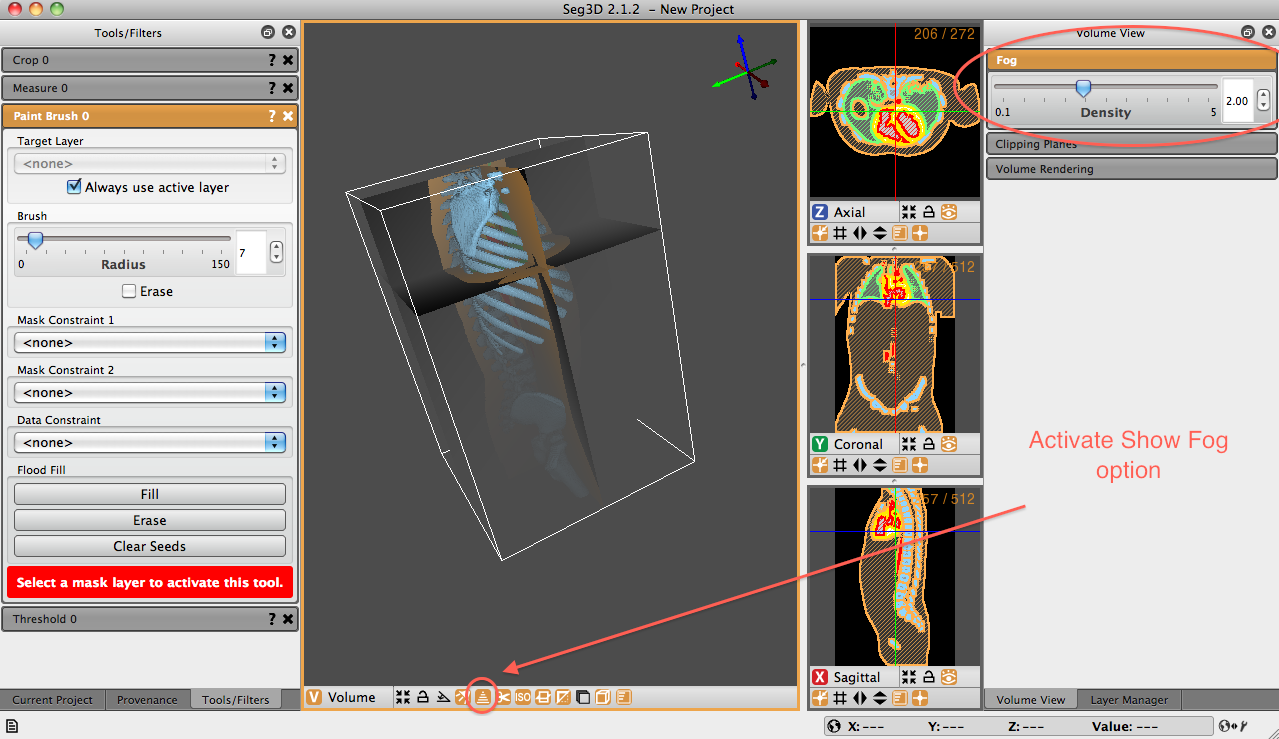
\includegraphics{Seg3DBasicFunctionality_figures/FogPanel.png}}
\caption{Volume View Window - Fog Panel Displayed. The user must activate the Show fog option at the bottom of the viewer window.}\label{fig:FogPanel}
\end{figure}

\subsection{Clipping Planes Panel}
\label{sec:clipping}
The Clipping Planes Panel allows users to define multiple clipping planes with which to clip the volume.  
+ and - signs at the top of the panel represent individual clipping planes.  
The + sign is an enabled clipping plan, while the - sign is disabled.
The clipping panel option in the viewer window is activated by default.

\begin{figure}[b!]
\scalebox{0.3}{\includegraphics{Seg3DBasicFunctionality_figures/ClippingPanel.png}}
\caption{Volume View Window - Clipping Panel Displayed. Show clipping option at the bottom of the viewer window is activated by default.}\label{fig:ClippingPanel}
\end{figure}

Once an clipping plane has been selected, it must be enabled.  Click the 'Enable' checkbox.  
After the plane is enabled, the user is able to define the influence of each cardinal direction on the plane.  
The number 1 in a box indicates that the clipping plane will slice a 45-degree angle within the positive side of that cardinal direction on the 3d viewing window. 
A -1 will clip a -45-degree angle from the negative side.

In order to activate a clip from any cardinal direction, the user must click the slider associated with the desired plane.
If the slider is not clicked, no clipping will take place...even with the clipping plane enabled.
If, say, the z slider is not clicked, no clipping will occur in that plane.
Combining these directional clips allows the user to define a plane that is tipped and tilted in any 3-dimensional direction.
A fourth slider option, the Distance slider, allows the user to define how the position of the clipping plane with respect to the volume.  
If the distance slider is set all the way to the left, no image will be displayed (it will be completely clipped).
If it is set to the right, the entire image will be displayed (no clipping is applied).  
Anything in between will show some clipping of the image.

The final option in the Clipping Planes panel is the option to 'Reverse Normal.'
This option allows the user to reflect the clipping plane.
That is, if the image is clipped within the positive XY plane, the 'Reverse Normal' option will display the clip within the negative XY plane
Figure \ref{fig:ClippingPanel} shows the result of a clipping plane applied in all three cardinal directions.

\subsection{Volume Rendering Panel}
\label{sec:volumerendering}
\begin{figure}[b!]
\scalebox{0.3}{\includegraphics{Seg3DBasicFunctionality_figures/VolRendPanel.png}}
\caption{Volume View Window - Volume Rendering Panel Displayed. Show volume rendering icon at the bottom of the viewer window must be activated.}\label{fig:VolRendPanel}
\end{figure}

The volume rendering panel allows users to generate a volume directly from the volume file, based on the application of transfer functions.
These volume representations are created by extracting values from the transfer functions available and displaying them on a slice-by-slice basis.
If the user zooms the image in closely, each individual slice can be seen (Figure \ref{fig:VolRendOpt}).
The user must define the volume over which they would like to perform the volume rendering.
The user must also make sure that the 'show volume rendering' option is selected at the bottom of the 3D viewer window.

\subsection{Rendering options}

With these two options selected, the user now has three rendering options.
These options are Simple, Faux Shading, and Ambient Occlusion.

\begin{figure}[h!]
\scalebox{0.3}{\includegraphics{Seg3DBasicFunctionality_figures/VolRendOpt.png}}
\caption{Volume Rendering Options - A) Simple B) Faux Shading C) Ambient Occlusion}\label{fig:VolRendOpt}
\end{figure}

\subsubsection{Simple}
The simple rendering strategy gives the user the option to select the Sapling Rate.
The higher the rate, the more accurate the representation of the selected region.
An option in the 'Transfer Function' section of the pane that allows the user to choose 'Solid' transfer function representation changes the appearance by coloring each selected slice to a solid color.
More on this feature will be addressed below.
Note that the images in Figure \ref{fig:VolRendOpt} do not have the solid option selected.

\subsubsection{Faux Shading}
Faux Shading is the same as the simple rendering option with the exception that a simple shading is added to the visible volume.
Where the simple rendering fades regions of the slice to clear (where the 'Solid' transfer function option is NOT selected), the Faux Shading options fade slices to a grayer hue, dependent on where it sits from other 3-dimensionally viewed volumes.
If the 'Solid' feature is selected, the Simple and Faux Shading rendering are the same.

\subsubsection{Ambient Occlusion}
Ambient Occlusion has several additional options.
In addition to the sampling rate, an occlusion angle (range: 0 to 80 degrees) and a sample resolution (range: 1 to 10) are now available.

%Not sure what is these additional options mean.
%The Sample Rate determines the general resolution of the volume.
%The Sample Resolution and the Occlusion angle determine


\subsection{Transfer Function}
Within the transfer function pane, a histogram exists that defines the volumetric image.
The transfer function can be displayed on a Linear or Logarithmic scale.
In the transfer function window, the user can choose to add or delete a feature.
A feature can be dragged into positions defining regions of the histogram that the user wants to render.
The default Feature is a line.  
By clicking and dragging the line, the feature can be moved.
By clicking a point on the line, the individual point can be moved.
Additional points can be added to a feature by clicking anywhere in the histogram panel  that is not already defined by a line, that is, in the gray or black regions.

Each of the features observed can also be enabled/disabled and viewed as solid or graded.
The solid feature (as addressed above) allows the feature to be represented as a graded slice or as a solid one.
Solid slices simply apply the same color saturation to each section of the volume slice.
De-selecting the solid option applies a gradient to the slices, with the outer edge being the brightest color.

Each point and feature can be repositioned, reshaped, and recolored in order to distinguish between defined regions.
To change the color of a feature, select the desired feature and adjust the slider regions below the histogram in the Red/Green/Blue features.
Colors can be used to easily distinguish different features in the volume.
Additionally, each features Ambient and Specular lighting can be adjusted as well as volume shininess is adjustable



\section{Provenance Window}
The Provenance Window is not opened by default when Seg3D is opened. 
To open the window, click the 'Window' option in the task bar and select the Provenance option.  
The window may also be toggled by using the key command: Shift+cntrl/cmd+H.
When the window opens, it will appear on the left side of the Seg3D user interface over top of the 'Current Project' panel and the 'Tools' panel.

The Provenance Window shows the history of the active layer.  
In order to see which actions lead to the current layer, highlight the layer in the 'Layer Window' on the left of the Seg3D display.
Initially, nothing will appear in the Provenance window.
Click the Refresh button at the bottom of the panel and the complete history of that mask will appear.

\begin{figure}[b!]
\scalebox{0.3}{\includegraphics{Seg3DBasicFunctionality_figures/ProvenanceWindow.png}}
\caption{Volume View Window - Clipping Panel Displayed. Show clipping option at the bottom of the viewer window is activated by default.}\label{fig:ProvenanceWindow}
\end{figure}

For example, Figure \ref{fig:ProvenanceWindow} shows an example of a 'FillHoles' Layer.
This layer was was generated by applying a FillHoles tool to the thresholded mask of the lungs.
As can be seen in the Provenance panel, the first step in creating this mask was to Import the volume layer.  
Next, a threshold was taken.  Last, the FillHolesFilter was applied to the Threshold mask.
By selecting one of the steps in the Provenance window, the parameters defining that portion of the mask history will be shown.
For example, by selecting the Threshold option, the thresholding range will be displayed.

\section{Controller Window}
The Controller Window is not opened by default when Seg3D is opened.  To open the window, click the 'Window' option in the task bar and select the Controller option.  The window may also be toggled by using the key command: Shift+cntrl/cmd+C.
Notice the Controller Window option in the window drop-down menu is located below a separator.  
This indicates that the window will open a new pop-up window outside of the general Seg3D user interface.

The Controller window supplies the user with all of the data, variables, history, and logs of the current Seg3D session.
There are four tabs that can be selected in this window:

\subsection{Actions Tab}
The action tab displays all of the actions that have been taken during the Seg3D session.
Console entries can also be made with this feature.
A series of actions area provided in a drop-down menu at the bottom of the window.
Once selected, the action will be placed into a command line to the right of the drop-down menu.
The user can then define the parameters for the action, or simply press enter to see what parameters are required to make the action valid.
If additional parameters are needed to run the action, they will be displayed in the box below the command line.

\subsection{State Variables Tab}
The state variables tab  shows a list of all the state settings for the session.
Settings cannot be edited in this window.

\subsection{Event Log Tab}
The event log shows actions that have been taken on the session since the latest load of the session.
If Seg3D is closed, and then reopened, the event log will only record the history for the newly opened session.
This differs from the action tab in this way, which collects actions for the entire history of the session.
The event log also differs from the action log in that it records all events involved with running Seg3D, not just the actions.
This is also a non-editable tab.

\subsection{Undo/Redo Buffer Tab}
The Undo/Redo Buffer stores past actions for the current open project.
Closing the session will erase the buffers.
In these buffers a user can find the actions, in order, than can be either undone or redone by using Seg3D's Undo and Redo options.


\section{Python Console}
The Python Window is not opened by default when Seg3D is opened.  To open the window, click the 'Window' option in the task bar and select the Python option.  The window may also be toggled by using the key command: Shift+cntrl/cmd+Y.
Notice the Python Window option in the window drop-down menu is located below a separator.  
This indicates that the window will open a new pop-up window outside of the general Seg3D user interface.

The Python Window opens a python scripting console that can be used by advanced users to editing the Seg3D data via python coding.  A treatment of python coding will not be attempted in this document.  For more information on python coding, consult other resources.

\section{Message History Window}
\label{sec:messagehistory}
The Message History Window is not opened by default when Seg3D is opened.  This window is opened by clicking on the message history icon in the bottom left of the screen in the tool bar (Figure~\ref{fig:messagehistory}).  This window will show the messages that Seg3D displays when many functions are performed.  This can be used to track your steps at a high level.  


%-------------------------------------------------


\chapter{Basic Program Functions}
\label{sec:functions}

\begin{introduction}
This section gives a brief overview of the options found under the File, Edit, and Help menus. These menus contain options
that allow you to save and open new projects, and set preferences. 

\end{introduction}

\section{File}
\label{sec:file}

\subsection{New Project}
\label{sec:newproject}
The new project option will prompt you to save your current project such that it can be closed. A dialog box will then open
asking for a Project name and a Project Path (Figure~\ref{fig:newproject}).  The Project name will be used to create a folder for all the project data.  The Project path defines the location of this folder, which can be set by typing the path or through a seperate dialogue box by pressing 'Choose Alternate Location'.  The default location for this path can be set in the preferences section discussed below. A new project can also be created using the shortcut cntrl/cmd+N.

\begin{figure}[h!]
\scalebox{0.6}{\includegraphics{Seg3DBasicFunctionality_figures/newProject.png}}
\caption{Project Information window is shown when a new project option is chosen. The project name and location are set in this window}\label{fig:newproject}
\end{figure}

\subsection{Open Project}
\label{sec:openproject}
The open project selection will prompt you to save you current project and open a new project based by selecting it from a file menu.  This function can be called using the shortcut cntrl/cmd+O.

\subsection{Show Project Folder}
This option will open a file menu showing the projects contained in your default project location.  This function can be called using the shortcut shift+cntrl/cmd+O.  The default project location can be changed in Seg3D preferences.

\subsection{Save Project}
If the project as already been given a name and location, this will save the project.  If the project has not yet been named, it will prompt the user for a project name and location.  This function can be called using the shortcut cntrl/cmd+S.

\subsection{Save Project As}
\label{sec:saveprojectas}
This will create a copy of the current project under a new name and project location.  This function can be called using the shortcut shift+cntrl/cmd+S.

\subsection{Launch Another Copy of Seg3D}
This opens a new session of Seg3D.  It does not close the current session, but simply opens another copy.

\subsection{Import Layer From Single File}
\label{sec:importsinglefile}
Data and label maps can be stored in a variety of file formats.  Use this option when the data or label map is stored in one single file.  This function can be called using the shortcut shift+cntrl/cmd+O.

\subsubsection{Import Widget}
After the user selects the file/files to be read, a menu will appear asking the user to define the type of data being read as seen below (Figure~\ref{fig:ImportWidget}).

\begin{figure}[h!]
\scalebox{0.6}{\includegraphics{Seg3DBasicFunctionality_figures/ImportWidget.png}}
\caption{When importing data or label masks, the user is prompted to define the type of data being read.}\label{fig:ImportWidget}
\end{figure}

There are two types of files that can be read by Seg3D: Image data and label maps.  The first selection indicates that the file you wish to read in contains image data.  The next three selections all apply to label maps.  The second selection assumes that all non-zero values are part of a single label map.  The third selection will define each unique value in the file as part of a separate label map. However, the numerical value assigned to represent that label will be incrementally generated by Seg3D rather than assigned from the input file. The fourth selection is similar to the third in that it creates labels based on unique values in the input file.  However, in this case the value used to represent the label is the same as the value being read from the file.

\subsection{Import Layer From Image Series}
Data and label maps can be stored in a variety of file formats.  Use this option when the data or label map is stored in multiple files. See Import Layer From Single File for more information about the Import Widget. This function can be called using the shortcut shift+cntrl/cmd+I.

\subsection{Export Segmentation}
Label maps can be exported in a variety of file formats.  If a layer containing a label map is selected, then the user may select the Export Segmentation option which opens the segmentation dialogue (Figure~\ref{fig:ExportSeg}).

\begin{figure}[h!]
\scalebox{0.6}{\includegraphics{Seg3DBasicFunctionality_figures/ExportSeg.png}}
\caption{This window appears when the user selects export segmentation.  It allows the user to select the layers they wish to export as label masks and the format they wish to export.}\label{fig:ExportSeg}
\end{figure}

This window allows the user to select the layers to export as label masks and the format they wish to export.  The available formats include: .nrrd, .mat (matlab), .tiff, .bmp, .png, .dcm. This function can be called using the shortcut cntrl/cmd+E.  The segmentation may be saved as a single file or as multiple files.  

After choosing a file name (single file only) and location for the segmentation, you will be shown the Export to Segmentation Summary.  This window shows the layers chosen to save as a segmentation.  In the case of saving as a single file,  there is an additional layer (the background, which is the remainder of the volume)  and an option to choose the value to represent each of the layers (Figure~\ref{fig:ExportSeg_2}).  I should be noted that the segmentation will only represent one value per voxel, so if any of the selected layers overlap the higher value will overwrite the region of overlap.  If saving as multiple files, this window will show the names of the layers only.  

\begin{figure}[h!]
\scalebox{0.6}{\includegraphics{Seg3DBasicFunctionality_figures/ExportSeg_2.png}}
\caption{This window appears when the user selects export segmentation and a file is chosen.  This allows the users to choose the labels to use for each material.  }\label{fig:ExportSeg_2}
\end{figure}

\subsection{Export Active Data Layer}

If image data layer is selected, then the user may choose to Export Active Data Layer. This selection opens a file menu window where the user can select the location they wish to save the data file as well as specify the file format.  The available formats include: .nrrd, .dcm, .tiff, .png, .mrc, and .mat (matlab). This function can be called using the shortcut shift+cntrl/cmd+E.

\subsection{Recent Projects}
This menu shows recently opened projects.  These projects can be opened quickly by clicking on the name of the project.

\section{Edit}

\subsection{Undo}
This function allows the user to undo a changes made to the unsaved project.  Changes made to the project are stored
in a buffer, the size of which can be changed under Seg3D preferences. This function can be called using the shortcut cntrl/cmd+Z.


\subsection{Redo}
Redo an operation on a project that was previously undone. This function can be called using the shortcut shift+cntrl/cmd+Z.


\subsection{Copy Mask Slice}
Copy a single slice from a mask layer which can then be pasted onto other layers. This function can be called using the shortcut cntrl/cmd+C.


\subsection{Paste Mask Slice}
Paste a previously copied label from one slice of a mask label to all the slices of another mask label. This function can be called using the shortcut cntrl/cmd+V.


\subsection{Punch Through Volume}
After creating new label data on a single slice of a mask layer, that label can be copied or "punched" to every other slice by
selecting this option. This function can be called using the shortcut cntrl/cmd+P.


\section{Help}
\subsection{Search}
This feature allows you to search all the menus by typing in a search box.

\subsection{Keyboard Shortcuts}
This function opens a list of all the keyboard and mouse shortcuts available in Seg3D.

\section{Preferences}
\label{sec:preferences}
The preference dialogue box can be opened by selection Seg3D-> preferences.  This dialog box
contains four tabs which we will discuss here.


\subsection{General}
The in Seg3D preferences, the general tab allows you to change many details of the "autosave" options.  The user
may turn on the autosave feature and set a frequency for which the project is save.  The "Don't interrupt me" option 
can be turned on so that the auto save does not happen while another operation is being performed. Along with the
frequency the amount of compression used to save each project can be controlled in this tab.  

The "import/export" options allows you to turn on an off a feature that will export a dicom header with all dicoms that are
exported.

The "project" options allow you to change the default project location, change the buffer size, and change how the project
is saved e.g. change if the input files are embedded into the project.

\begin{figure}[h!]
\scalebox{0.6}{\includegraphics{Seg3DBasicFunctionality_figures/Pref_gen.png}}
\caption{The Seg3d preferences under the general tab.}\label{fig:Pref_gen}
\end{figure}


\subsection{View}
Under this tab the user is able to change many of the default view options such as the window layout (1 big window with 3 smaller windows), background color, and Grid size. In addition there are many options to customize what is seen in the visualization window.  At the bottom of this window the user can change the axis labels such that the X,Y, and Z directions
are not fixed to represent Sagittal, Coronal, and Axial, but the user can define which axis label is assigned to each direction.

\begin{figure}[h!]
\scalebox{0.6}{\includegraphics{Seg3DBasicFunctionality_figures/Pref_view.png}}
\caption{The Seg3d preferences under the view tab.}\label{fig:Pref_view}
\end{figure}

\newpage

\subsection{Layers}
Under this tab the user can change the appearance of the label masks. These options include: layer opacity, available colors, mask fill option (striped or solid), and border thickness.

\begin{figure}[h!]
\scalebox{0.6}{\includegraphics{Seg3DBasicFunctionality_figures/Pref_layers.png}}
\caption{The Seg3d preferences under the layers tab.}\label{fig:Pref_layers}
\end{figure}


\subsection{Sidebars/Tools + Filters}
Under this tab the user can select which menus appear on start up and which tools/filters will appear in the 
sidebars.  This intended for the user to customize their user interface to improve the ease of use.

\begin{figure}[h!]
\scalebox{0.6}{\includegraphics{Seg3DBasicFunctionality_figures/Pref_side.png}}
\caption{The Seg3d preferences under the sidebars/tools + filters tab.}\label{fig:Pref_side}
\end{figure}



%-----------------------------------------------------------------------



\chapter{Tools \& Filters}
\label{sec:tools_filters}

\begin{introduction}

\end{introduction}

\section{Tools}

\subsection{Copy/Paste}

\subsection{Crop}

\subsection{etc.}

\section{Mask Filters}

\subsection{etc.}

\section{Data Filters}

\subsection{etc.}

\section{Advanced Filters}

\subsection{etc.}

\end{document}

